\documentclass[10pt]{article}
\usepackage[utf8]{inputenc}
\usepackage{amsmath}
\usepackage{amsfonts}
\usepackage{amssymb}

% package used to enabled option of no-spacing in itemized lists
\usepackage{enumitem}

% this is to make it look like a word document.
\usepackage[tmargin=0.98in,bmargin=0.98in,lmargin=1.18in,rmargin=1.18in]{geometry}

% package necessary to add pictures to latex
\usepackage{graphicx}

% package needed to draw a frame for a text
\usepackage[linewidth=1pt]{mdframed}

% needed packages for using algorithms
\usepackage{algorithm,algorithmicx,algpseudocode,float}

\title{\vspace{-4ex}\textbf{Algoritmo de Dijkstra}\vspace{-2ex}}
\date{\today}
\author{Luis Servín\\ Taller TRA, Universidad Nacional Autónoma de México}

\begin{document}

\maketitle

Si se considera la situación mostrada en la figura \ref{fig:situation1} en la cual tenemos un objeto que va a desplazarse a través de su entorno. A continuación se ejemplifican dos situaciones que pueden presentarse:
\begin{itemize}
	\item El objeto sigue una trayectoria directa hacia la meta. Ya que no existe indicio de que no deba seguir esta ruta debido a las lecturas del área que puede escanear (área roja) avanza con confianza. Cerca de la meta detecta un obstáculo y decide cambiar de dirección para evadirlo. Durante su movimiento descubre que se trata de un obstáculo en forma de "U", por lo cuál tuvo que realizar la trayectoria roja punteada mucho mas largo de lo previsto inicialmente.
	
	\item Previo a comenzar a moverse, el sistema obtiene un conocimiento del ambiente que lo rodea (área azul). Con base en esta información utiliza un algoritmo de planificación de ruta para encontrar un camino mas corto hacia la meta, y así evitar obstáculos en el ambiente.
\end{itemize}

\begin{figure}[h!]
	\centering
	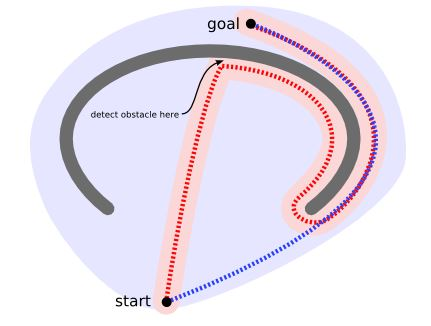
\includegraphics[scale=0.5]{images/situationPathFinding.JPG}
 	\caption{Ventaja de contar con una planeación de ruta previa}
	\label{fig:situation1}
\end{figure}

Gracias a lo descrito anteriormente podemos notar una de las principales ventajas de los algoritmos de planeación de ruta; Estos te permiten realizar un plan de las acciones a tomar con base en la información actual del ambiente, en lugar de esperar hasta el último momento para descubrir que existe un problema. Aunque la planeación anticipada suele ser mas lenta que los comportamientos reactivos llega a producir mejores resultados, si es que el ambiente no ha cambiado de manera drástica. Por lo tanto con el objetivo de aprovechar lo mejor de ambas propuestas, se recomienda utilizar ambos: Un planificador de ruta que tome en cuenta la información global en caminos largos; y un algoritmo reactivo para movimientos rápidos en situaciones no previstas en un inicio.

Estos algoritmos de planeación trabajan sobre gráficas, que se pueden definir como un conjunto de vértices con aristas que los conectan entre sí. Basándonos en esto podemos establecer una gráfica a partir de un mapa cuadriculado como el que se muestra en la figura \ref{fig:gridmap}. Este podemos definir a cada unidad o cuadro como un vértice y establecer una arista entre dos unidades continuas que comparten un lado. Con base en la información anterior podemos aplicar un algoritmo de planeación de ruta sobre un mapa cuadrículado como los el algoritmo de Dijkstra.

\begin{figure}[!]
	\centering
	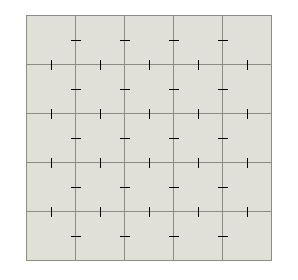
\includegraphics[scale=0.5]{images/gridMap.JPG}
 	\caption{Representación de un mapa cuadriculado (grid-map)}
	\label{fig:gridmap}
\end{figure}

El algoritmo de Dijkstra resuelve el problema de encontrar la ruta mas corta de un punto dentro de la gráfica (la fuente) hacia un punto objetivo. Este algoritmo fue diseñado por el científico Edsger W. Dijkstra en 1956. Aunque en primera instancia el algoritmo puede encontrar el camino mas corto entre dos puntos dentro de la gráfica, una variante mas común consiste en establecer un punto como inicial y a partir del mismo encontrar la ruta mas corta a todos los puntos dentro de la gráfica.

EL algoritmo trabaja al visitando los vértices dentro de la gráfica comenzando en el punto inicial. Enseguida de manera repetitiva examina los vértices mas cercanos que no hayan sido visitados aún, añadiéndolos al conjunto de objetos que han sido visitados. De esta manera se expande desde el punto inicial hasta que encuentra el punto objetivo. Además tiene como característica que puede garantizar encontrar la ruta mas corta entre ambos puntos, siempre y cuando ninguna de las conexiones tenga un peso negativo.

Una vez explicado el proceso a seguir de manera sencilla, procedemos formalizar el proceso



% -------------------------------------------------- %
% DESCRIPCIÓN GENERAL DEL ALGORITMO
% -------------------------------------------------- %


\begin{mdframed}

Sea el nodo en el cual comenzamos conocido como \textbf{nodo inicial}. Ahora sea la \textbf{distancia del nodo Y} la distancia actual entre el nodo inicial y el nodo Y. Como primer paso se asignara un valor de distancia inicial, la cual se tratará de mejorar de manera iterativa.

% COMIENZA LA DESCRIPCIÓN DE LOS PASOS DENTRO DEL NODO

\begin{enumerate}[]

	\item Asignar a cada nodo un valor inicial de distancia. Establecer un valor de cero para nuestro nodo incial e infinito para todos los demás.
	
	\item Establecer el nodo inicial como el actual. Los nodos restantes se establecerán como no visitados. Crear un conjunto que contenga todos los nodos no visitados conocido como \emph{unvisited}.
	
	\item \label{it:iterativeInitial} Para el nodo actual, considerar todos los vecinos o nodos con un conexión directa que se encuentren dentro del conjunto \emph{unvisited} y calcular su distancia tentativa. Compara la distancia tentativa obtenida con la que esta asignada hasta el momento, mantener el valor mas pequeño.
	
	\item Una vez que se hayan calculado las distancia a todos los nodos vecinos, marcar el nodo actual como \emph{visitado} y eliminarlo del conjunto \emph{unvisited}. Un nodo que haya sido marcado como visitado no volverla a ser analizado de nuevo.
	
	\item Si el nodo objetivo ha sido marcado como visitado (en caso que se busque una ruta entre dos nodos específicos) o si la distancia tentativa mas pequeña entre los nodos del conjunto \emph{unvisited} es infinito (en caso de que no haya una conexión entre el nodo inicial y los nodos restantes) deternerse.
	
	\item De lo contrario, seleccionar el nodo que tiene la distancia tentativa mas pequeña dentro del conjunto \emph{unvisited}. Establecerlo como nodo inicial y regresar al paso \ref{it:iterativeInitial}
	
\end{enumerate}

\end{mdframed}

% -------------------------------------------------- %
% FIN DE LA DESCRIPCIÓN
% -------------------------------------------------- %

Una vez descrito el algoritmo, se establece un \textbf{pseudocódigo} que puede servir como base para implementar dicho algoritmo en un lenguaje de programación.

\begin{algorithm}[H]
\begin{algorithmic}
\Function{Dijsktra}{Graph, Source} \\
	\quad create vertex set Q \\
	\quad \textbf{for each} vertex v in Graph: \Comment{Initialization} \\
		\qquad $dist[v] \gets$ INFINITY \Comment{Unknown distance from source to v} \\
		\qquad $prev[v] \gets$ UNDEFINED \Comment{Previous node in optimal path from source} \\
		\qquad add v to Q \Comment{All nodes initially in Q (unvisited nodes)} \\
	\quad $dist[source] \gets 0 $ \Comment{Distance from source to source} \\
	\quad \textbf{while} Q is not empty: \\
		\qquad $u \gets$ vertex in Q with min dist[u] \Comment{Source code will be selected first} \\
		\qquad remove u from Q \\
		\qquad \textbf{for each} neigbor v of u: \Comment{where v is still in Q} \\
			\quad \qquad $alt \gets$ dist[u] + length(u,v) \\
			\quad \qquad \textbf{if} $alt < dist[v]$ \Comment{A shorter path to v has been found} \\
				\qquad \qquad $dist[v] \gets alt$ \\
				\qquad \qquad $prev[v] \gets u$ \\
	\quad \textbf{return} dist[], prev[]
\EndFunction
\end{algorithmic}
\end{algorithm}


\end{document}













